\section{Applications}

The functionality and usability of \biochem is best demonstrated with examples. We chose three small scenarios, we begin with a simple example to show how some of the core structures can be created and used. Then we had over to a more complex example where we want to compare two different configurations of the same molecule. Finally, we want to demonstrate the elegance of Julia written code in comparison to C++. In the last application, we briefly introduce the accompanying visualization tool \bioviz that has been developed alongside the \biochem framework.

\subsection{Generating a water molecule}

The class diagramm in Figure~\ref{fig:biochem_uml} shows the core of \biochem. The interface is intuitively designed and the interactions with the components are straightforward as can be seen in code listing~\ref{lst:code-water}. The center of an application is the \texttt{System}. If no such system is explicitely created a default system is generated. Atoms can be created and the corresponding bonds and will automatically be part of the defined system. The names of the classes for the molecular entities and related functionalities were carefully chosen to be as intuitive as possible. The resulting system with the contained water molecule can be visualized via the visualization tool \bioviz. See Figure~\ref*{fig:biochem_water} and the following sections for more details. 
\begin{lstlisting}[
language = Julia, 
numbers=left, 
label={lst:code-water}, 
caption={Intuitive usage of \biochem core components}
]
using BiochemicalAlgorithms
using BiochemicalVisualization

sys = System() 
h2o = Molecule(sys)

o1 = Atom(h2o, 1, Elements.O)
h1 = Atom(h2o, 2, Elements.H)
h2 = Atom(h2o, 3, Elements.H)

h1.r = [1, 0, 0]
h2.r = [cos(deg2rad(105)), sin(deg2rad(105)), 0]

Bond(h2o, o1.idx, h1.idx, BondOrder.Single)
Bond(h2o, o1.idx, h2.idx, BondOrder.Single)

println("Number of atoms: ", natoms(h2o))
println("Number of bonds: ", nbonds(h2o))

ball_and_stick(sys)	
stick(sys)
van_der_waals(sys)
\end{lstlisting}


\subsection{RMSD computation and Application of Amber}

A very common task in structural analysis is the comparison of two or more structures. The following example will demonstrate the entire molecular pipeline. First, the two pdb files are loaded into a system container. Compared to the previous example, the variable \texttt{sys} represent a \texttt{Vector} of \texttt{Systems} instead of a single system. The systems are preprocessed with the \texttt{FragmentDB}, a database containing known fragments of molecules. The preprocessing steps include the normalization of different naming standards, the reconstruction of missing parts of the molecules and the creation of bonds, since pdb format usually contain no or incomplete bond information.  After the preprocessing, the molecular structures are each applied to a molecular force field and here the amber energy of the systems are computed. The structures studied in this example are different configuration of the same molecule and can be mapped onto each other. Before and after the mapping the RMSD is computed and displayed.  \\
This example demonstrates the rich functionality of \biochem by just a few lines of code. The steps that were carefully taken to prepare the systems are shown in Figure\ref{fig:biochem_visualization}.
\begin{lstlisting}[
    language = Julia, 
    numbers=left, 
    label={lst:rmsd-and-amber}, 
    caption={Comparison and mapping of two similar structures}
]
sys = load_pdb.(["data/arnd1.pdb", 
				 "data/arnd2.pdb"])

fdb = FragmentDB()
normalize_names!.(sys, Ref(fdb))
reconstruct_fragments!.(sys, Ref(fdb))
build_bonds!.(sys, Ref(fdb))

println.(sys)

compute_energy.(AmberFF.(sys), verbose=true)

println("RMSD before mapping: ", 
		compute_rmsd(sys[1], sys[2]))

map_rigid!(sys[1], sys[2])

println("RMSD after mapping: ", 
		compute_rmsd(sys[1], sys[2]))
\end{lstlisting}

\todo{output?}
\subsection{A trivial comparison between C++ and Julia}

The verbose nature of C++ comes apparent in a simple task. A typical situation in molecular simulation is to find out, which atoms are in a certain proximity of each other. As these atoms can exert interactions, which are important for the stability of a structure configuration. We would solve this task with advanced data structures such as a hash grids. However, for simplicity, we consider the following task: We want to count the contacts between two separate molecules, that are in close proximity. We will define a contact, if the distance between two carbon atoms $C_\beta$ atoms is smaller than $6$\AA. \\

The code listing below shows the solution for the task in C++. It is important to note here, that due to readability, the necessary includes for this even short code snippet are not shown. Using two nested for-loops, possible $C_\beta$ atoms are searched, whose distance from each other is computed in the next step. \\
In contrast, with \biochem this task is solved much
\begin{figure*}
\begin{lstlisting}[
	language = C++, 
	numbers=left, 
	label={lst:code-c++}, 
	caption={The resulting C++ code for the example task consist of a lot of boilerplate code.}
	]
int count_contacts(const AtomContainer& ac1, const AtomContainer& ac2, double thres = 6.0) {
	auto contacts = 0;
	for(auto ait1 = ac1.beginAtom(); +ait1; ++ait1) {
		if(ait1->getName() != "CB")
		continue;
		
		for(auto ait2 = ac2.beginAtom(); +ait2; ++ait2) {
			if(ait2->getName() != "CB")
			continue;
			
			auto dist = ait1->getPosition().getDistance(ait2->getPosition());
			if(dist <= thres) {
				contacts++;
			}
		}
	}
	return contacts;
}
\end{lstlisting}
\end{figure*}


\begin{figure*}
\begin{lstlisting}[
	language = Julia, 
	numbers=left, 
	label={lst:code-task-julia}, 
	caption={The resulting Julia code for the example task is much more elegant.}
	]
using BiochemicalAlgorithms 
	
function filter_cbeta(ac::AbstractAtomContainer{Float32})
	(atom for atom in atoms(ac) if atom.name == "CB")
end
	
function is_in_contact(r1::Vector3{Float32}, r2::Vector3{Float32})
	distance(r1, r2) <= 6
end
	
function count_contacts(ac1::AbstractAtomContainer{Float32}, ac2::AbstractAtomContainer{Float32})
	count( t -> is_in_contact(t...), ((a1.r, a2.r) for a1 in filter_cbeta(ac1), a2 in filter_cbeta(ac2)))
end
\end{lstlisting}
\end{figure*}

\subsection{Visualization using \bioviz}

A key feature of \biochem is the visualization tool \textit{\bioviz} that
has been developed alongside the main framework. As shown in Figure~\ref{fig:biochem_water} \ \bioviz currently supports three different representation of atomic structures, namely \texttt{ball-and-stick}, \texttt{van-der-Waals} and \texttt{stick} (cf. code listing~\ref{lst:code-water}).

When dealing with three dimensional structures of macromolecules, visualization plays an important role for supporting the development of insights into molecular functions. The possibility to visualize and interactively modify the representations provides great support during modelling scenarios. For instance, the tool has been used to visualize different steps from code listing~\ref{lst:rmsd-and-amber}. The first image left represent the raw input read from the underlying pdb file, the image in the middle shows the same input after preprocession it with the fragment data base (lines4-7). Finally, the mapping of both structures is shown in the image on the left. As can be seen, the structures do not match perfectly onto each other. 

Even this rather simple example already demonstrates the advantage of a visual representation that can be modified and manipulated in context of modelling scenarios and how the visualization supports the development of knowledge of molecular functions.

 \begin{figure*}[t]
	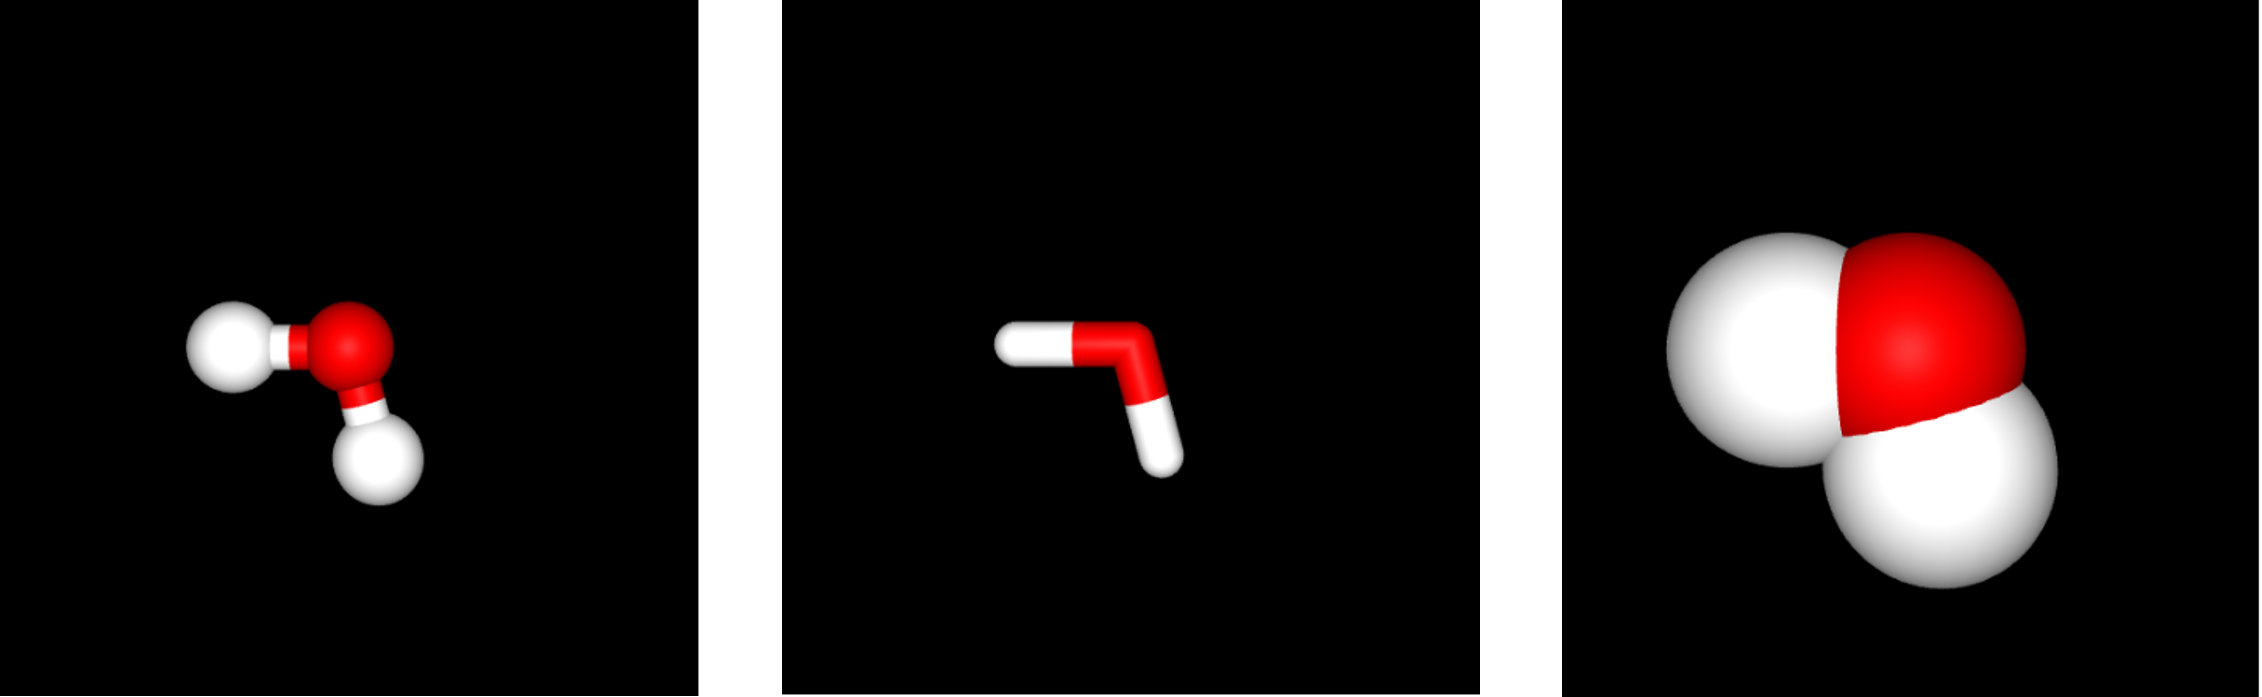
\includegraphics[width=18cm]{gfx/biovis-2.png}
	\caption{\bioviz supports three models:  \texttt{ball-and-stick} \textit{(left)}, \texttt{stick} \textit{(center)} and \texttt{van-der-waals} \textit{(right)} representation of the water molecule as generated by the code listing~\ref{lst:code-water}.}
	\label{fig:biochem_water}
\end{figure*}

\begin{figure*}[t]
	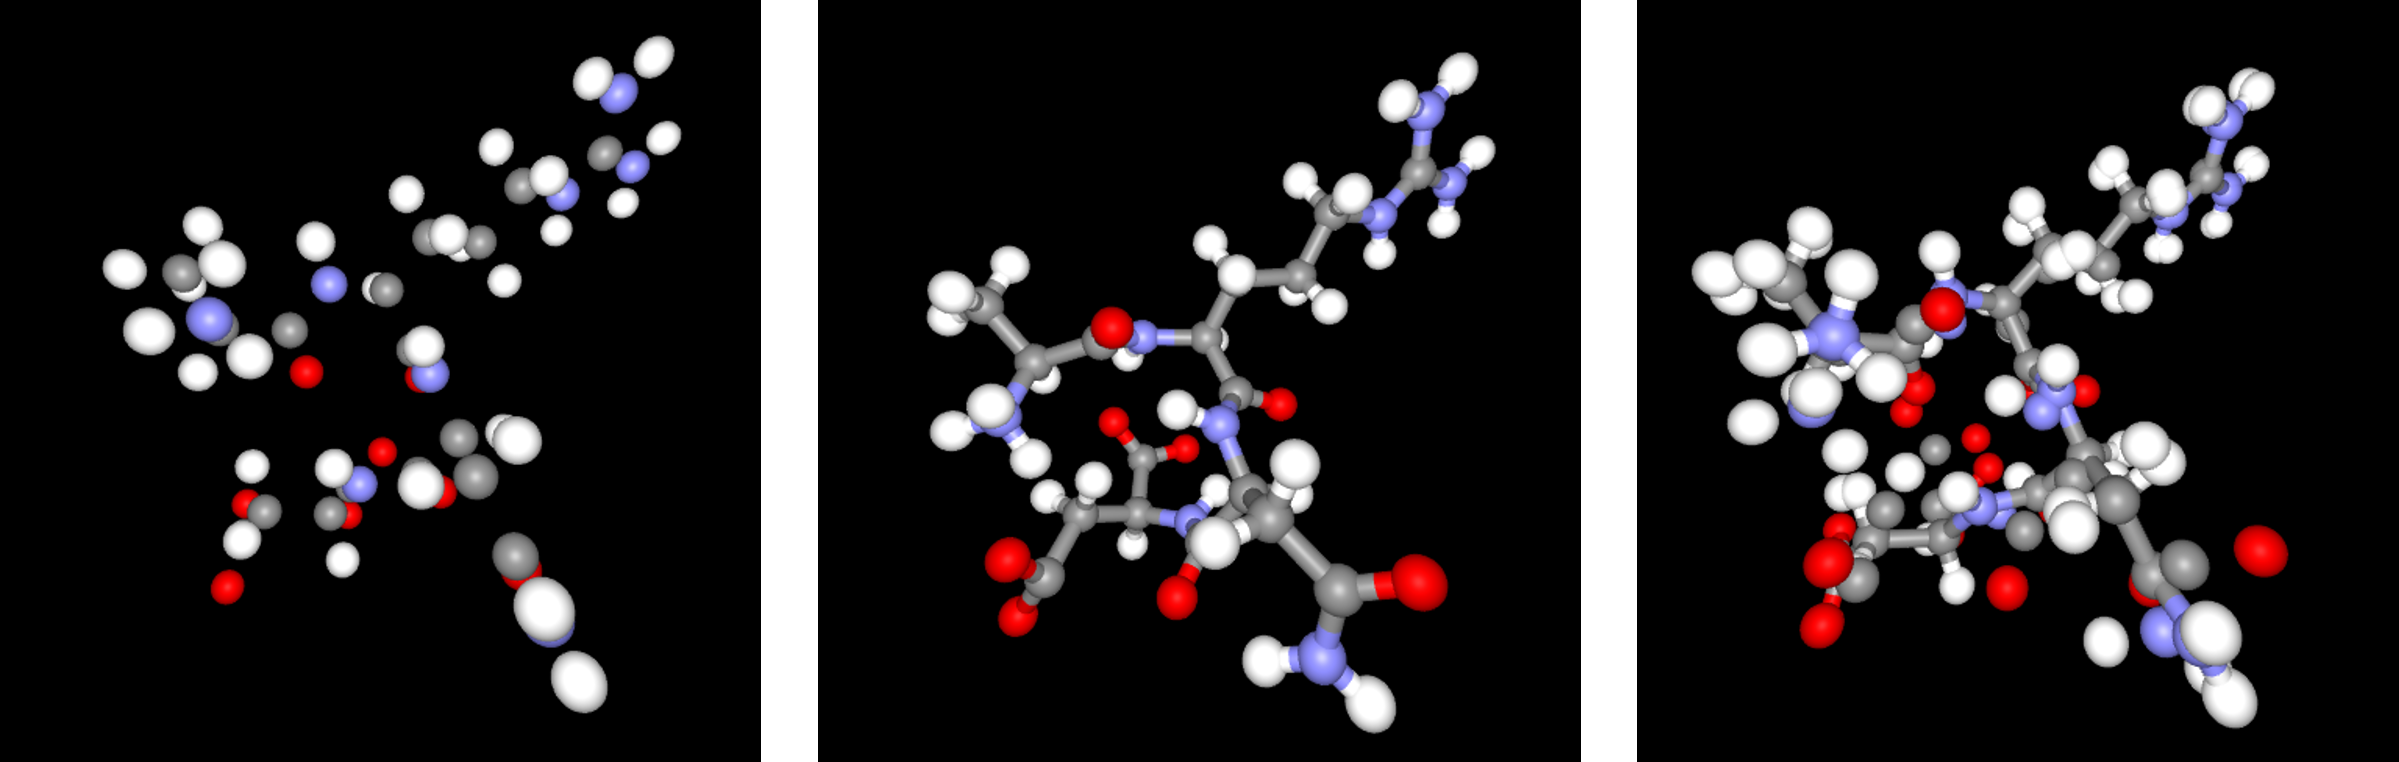
\includegraphics[width=18cm]{gfx/biovis.png}
	\caption{The \texttt{ball-and-stick}-representation of the code listing~\ref{lst:rmsd-and-amber}. The first molecule without preprocessing (\textit{left}) and after preprocessing (\textit{center}). Finally, the two structures are superposed (\textit{right}).}
	\label{fig:biochem_visualization}
\end{figure*}